% Anexos
\appendix
\clearpage
\addappheadtotoc
\appendixpage

\fancyhead[LO]{\small ANEXOS}
\fancyhead[RE]{\small ANEXOS}

\chapter{Aspectos éticos, económicos, sociales y ambientales } \label{anx:et}
  En este anexo se va a realizar una descripción de los aspectos éticos, económicos, sociales y ambientales surgidos de la realización del trabajo. 

\section*{Introducción}
  Este trabajo de fin de grado está integrado en el proyecto COBRA de la ETSIT, y su objetivo es optimizar la forma en la que se realiza actualmente el despliegue de los Cyber Range, en términos de velocidad, escalabilidad, portabilidad y seguridad. 

  Desde un punto de vista social, el principal colectivo afectado o asociado a la realización de este proyecto estaría estrechamente relacionado con el ámbito de la ETSIT. Considerando los planos económico, medioambiental y ético, el trabajo aporta valor en todos ellos, tal y como se va a detallar a continuación. 

\section*{Impactos relacionados con el proyecto}
  En primer lugar, el sistema desarrollado proporcionará una mayor productividad y calidad en la formación de los alumnos que cursen asignaturas de ciberseguridad así como programas de estudios relacionados con ella. Como ya se ha comentado en secciones anteriores, el despliegue en la nube supone un gran ahorro económico, ya que se paga únicamente por los recursos que se usan y durante el tiempo que se usan, de forma que en el caso de que no hubiera nadie practicando, no habría costes asociados. Además, es un entorno seguro, pues los escenarios son desplegados en una infraestructura completamente independiente del entorno de la organización, lo cual evita cualquier conflicto ético al no haber información o recursos sensibles de por medio\dots

  En cuanto al plano medioambiental, y estrechamente relacionado con el económico ya comentado, esta herramienta evita la compra innecesaria de dispositivos específicos para su empleo y uso. Esto se debe a que el sistema está completamente virtualizado, y por tanto es posible su despliegue completo en la nube, siendo por tanto compatible con cualquier tipo de ordenador, con independencia de su sistema operativo. Este aspecto permite reducir la huella ambiental al reducir los residuos a largo plazo.

  Adicionalmente, al estar el proyecto COBRA ligado al programa de gobierno COINCIDENTE, el sistema tendrá gran importancia de cara a la sociedad española, pues unos resultados positivos derivados del éxito del trabajo permitirían una mejor formación en los profesionales de ciberseguridad de España, lo que a su vez mejoraría la calidad de vida de las personas.

\section*{Análisis detallado de uno de los principales impactos}
  Tras la exposición en la sección anterior de los impactos más relevantes relacionados con el proyecto, podemos afirmar que uno de los más influyentes sería el plano económico-medioambiental asociado al despliegue en Cloud. 

  El hecho de poder virtualizar cualquier tipo de sistema proporciona una gran flexibilidad a la hora de definir escenarios completamente distintos entre sí y evita la compra de equipos específicamente para ello. Un Cyber Range que se despliega haciendo uso de equipos físicos corre el riesgo de que haya periodos de tiempo en los que no se use, lo cual no exime del pago de la infraestructura que se emplea. Mientras tanto, en la nube tanto el despliegue como el pago de la infraestructura es bajo demanda.

  Además, respecto al uso de GCP como proveedor cloud, cabe destacar que Google no tiene emisiones de carbono desde 2007 y se comprometió a operar con energía neutra de carbono en un 100\% las 24 horas, todos los días, para el año 2030. Los centros de datos de Google, incluidos los que ejecutan los servicios de Google Cloud, también usan mucho menos energía que los centros de datos típicos. Por este motivo, el uso de Google Cloud ayuda a reducir la huella de carbono de la infraestructura IT.

\section*{Conclusiones}
  A lo largo del desarrollo del proyecto se han realizado decisiones sobre requisitos y objetivos a cumplir que han sido claves para el alcance de un ecosistema que favorece al desarrollo sostenible y a la mejora de la sociedad. 

  Es por esto que podemos llegara a la conclusión de que todas las personas y organizaciones involucradas en el proyecto obtienen un beneficio e impacto positivo como consecuencia del uso del sistema desarrollado. 

\chapter{Presupuesto económico} \label{anx:ec}
  Este anexo presenta una estimación de los costes asociados a la realización de este trabajo de fin de grado y que han sido necesarios para la consecución de los objetivos. Se van a tener en cuenta para ello tanto los materiales utilizados como la mano de obra, a partir de los cuales se realizará una aproximación de los costes directos e indirectos. 

\section*{Costes de mano de obra}
  Para estimar el coste asociado a la mano de obra, en primer lugar se ha realizado una aproximación del número de horas empleadas en las diferentes etapas de realización del proyecto. Esta aproximación se muestra con detalle en la tabla inferior. 
  
  \begin{table}[h]
    \begin{center}
      \begin{tabular}{ | m{13,5cm} | w{c}{1,5cm} | }
        \hline\rowcolor{oranget} \centering\textbf{Subproceso} & \textbf{Horas} \\ \hline
        Estudio de las diferentes tecnologías (Terraform, Google Cloud) & 90 \\ \hline\rowcolor{oranger}
        Análisis de los escenarios (vector de ataque y conexiones necesarias entre los elementos) & 40 \\ \hline
        Diseño e implementación de los escenarios en Google Cloud & 130 \\ \hline\rowcolor{oranger}
        Desarrollo de herramientas de configuración & 30  \\ \hline\
        Pruebas & 40  \\ \hline\rowcolor{oranger}
        Elaboración de la memoria & 75 \\ \hline\rowcolor{total}
        \textbf{Total} & \textbf{405} \\ \hline
      \end{tabular}
      \caption{Horas asociadas a cada una de los subprocesos de realización del proyecto}
      \label{tab:hours}
    \end{center}
  \end{table}
  
  Una vez obtenida una aproximación de las horas empleadas en todo el proceso de diseño y desarollo del sistema, se va a considerar el salario medio anual de un Ingeniero de Telecomunicación junior para estimar el coste de mano de obra. Según el informe llevado a cabo por el Colegio Oficial de Ingenieros de Telecomunicación (COIT) en su Mapa socio-profesional del titulado en Ingeniería de Telecomunicación~\cite{anx1}, el salario medio anual de los titulados entre 18 y 24 años es de 23.553€, que con un contrato de 40h semanales y estimando 48 semanas laborales anuales resultaría en 12.27€/hora. Con este dato podemos finalmente estimar el coste de la mano de obra:

  \begin{table}[h]
    \begin{center}
      \begin{tabular}{ | c | c | c | }
        \hline \hline
        \multicolumn{3}{c}{Costes de mano de obra} \\ \hline \hline
        \hline \centering\textbf{Horas}\cellcolor{oranget} & \textbf{€/Hora}\cellcolor{oranget} & \textbf{Total}\cellcolor{total} \\ \hline
        405 & 12.27 & \textbf{4.969,35€}\cellcolor{total} \\ \hline
      \end{tabular}
      \caption{Costes de mano de obra}
      \label{tab:man}
    \end{center}
  \end{table}

\section*{Costes materiales}
  Para los costes materiales se tendrá en cuenta el ordenador personal con el que se ha realizado todo el desarrollo. Dicho equipo es un HP Pavilion 15-cs0012ns, que cuenta con un procesador Intel Core i7, una pantalla de 15.6" y 16GB de memoria RAM como algunas de sus características principales. Este ordenador tiene un coste aproximado de 1.100€. Además, se ha calculado la amortización mensual en base a los 4 años de antigüedad que tiene y esta se ha multiplicado por el número de meses en los que se ha estado trabajando en el proyecto (Octubre-Junio) para obtener la amortización total.

  También se ha de tener en cuenta que para la simulación de los escenarios fue necesario el uso de servicios de GCP que quedan fuera de la capa gratuita que ofrece Google y que por tanto tienen un coste asociado al tiempo que se han usado durante el desarrollo y las pruebas. En la imagen inferior se adjunta un reporte de los gastos en dichos servicios a lo largo del tiempo, acompañados del montante total. 

  \begin{figure}[h]
  \centering
  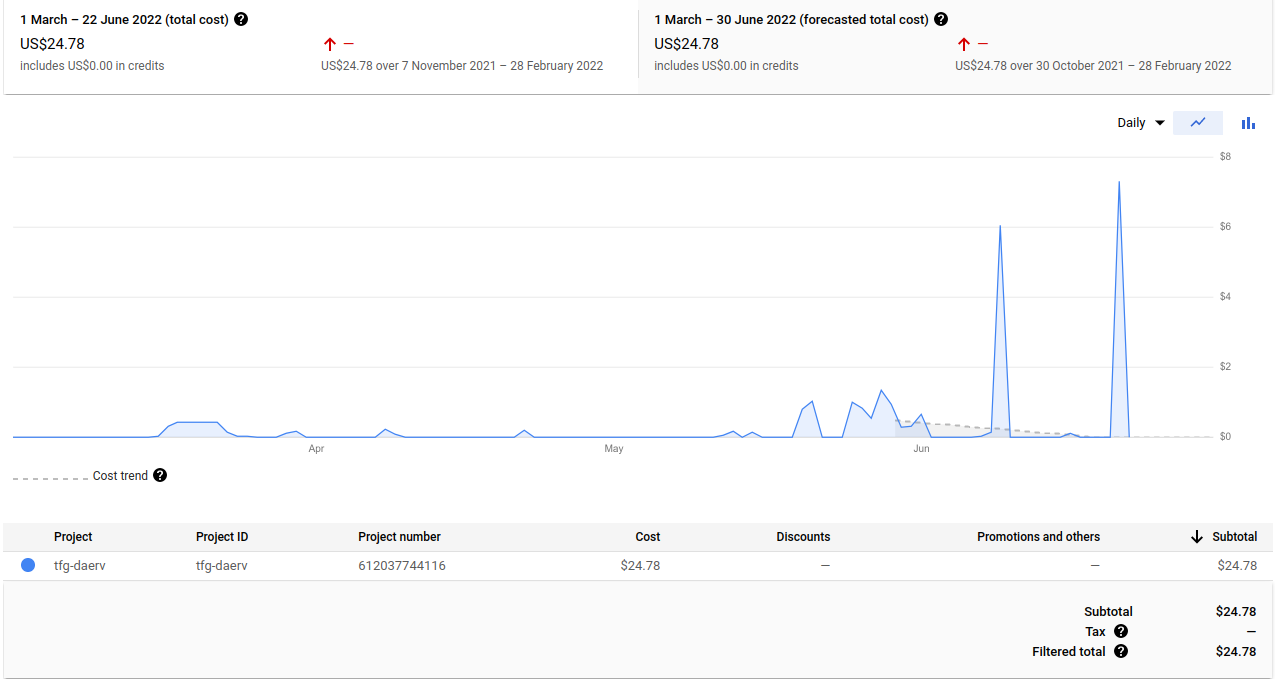
\includegraphics[width=\textwidth]{../imgs/desarrollo/facturacion/graph.png}
  \caption{Resumen de pagos en servicios de GCP}
  \end{figure}

  Como se puede apreciar, el gasto total ha sido de 24.78\$, que con la equivalencia actual (1€=1.06USD) serían 23,41€. Este dato nos permite cerrar los costes materiales como se puede ver a continuación.

  \clearpage
  \begin{table}[t]
    \begin{center}
      \begin{tabular}{ | c | m{2,5cm} | c | m{2,75cm} | m{1,75cm} | c | }
        \hline \hline
        \multicolumn{6}{c}{Costes materiales} \\ \hline \hline
        \hline \centering\textbf{Material}\cellcolor{oranget} & \textbf{Tiempo de vida (años)}\cellcolor{oranget} & \textbf{Precio}\cellcolor{oranget} & \centering\textbf{Amortización (€/mes)}\cellcolor{oranget} & \centering\textbf{Uso (meses)}\cellcolor{oranget} & \textbf{Total}\cellcolor{oranget} \\ \hline
        Ordenador portátil & \centering4 & 1.100€ & \centering22.92 & \centering8 & \textbf{183,36€} \\ \hline\rowcolor{oranger}
        Servicios GCP & \centering- & 23,41€ & \centering- & \centering- & \textbf{23,41€} \\ \hline\rowcolor{total}
        \multicolumn{5}{|c|}{\textbf{Total}} & \textbf{206,77€} \\ \hline
      \end{tabular}
      \caption{Costes materiales}
      \label{tab:mat}
    \end{center}
  \end{table}
    
\section*{Costes indirectos}
  Se han estimado los costes indirectos (como pueden ser luz, agua o internet) en un 20\% sobre la suma de los costes de mano de obra y material:
  
  \begin{table}[h]
    \begin{center}
      \begin{tabular}{ | c | c | c | }
        \hline \hline
        \multicolumn{3}{c}{Costes indirectos} \\ \hline \hline
        \hline \centering\textbf{Coste directo}\cellcolor{oranget} & \textbf{Estimación}\cellcolor{oranget} & \textbf{Total}\cellcolor{total} \\ \hline
         5.176,12€ & 20\% & \textbf{1.035,224€}\cellcolor{total} \\ \hline
      \end{tabular}
      \caption{Costes indirectos}
      \label{tab:ind}
    \end{center}
  \end{table}

\section*{Costes totales}
  Para terminar, se incluyen el IVA y el beneficio industrial para obtener los costes totales asociados al proyecto:

  \begin{table}[h]
    \begin{center}
      \begin{tabular}{ | c | c | c | }
        \hline \hline
        \multicolumn{3}{c}{Costes totales} \\ \hline \hline
        \hline \multicolumn{2}{|c|}{\textbf{Concepto}\cellcolor{oranget}} & \textbf{Coste}\cellcolor{oranget} \\ \hline
        \multirow{3}{*}{Costes directos} & Mano de obra & 4.969,35€ \\ \cline{2-3} 
         & Material & 206,77€ \\ \cline{2-3} 
         & \textbf{Total} & \textbf{5.176,12€} \\ \hline\rowcolor{oranger}
        \multicolumn{2}{|c|}{Costes indirectos} & 1.035,22€ \\ \hline
        \multicolumn{2}{|c|}{Total antes de beneficios e impuestos} & 6.211,34€ \\ \hline\rowcolor{oranger}
        \multicolumn{2}{|c|}{Beneficio industrial (10\%)} & 621,13€ \\ \hline
        \multicolumn{2}{|c|}{Total antes de impuestos} & 6.832,48€ \\ \hline\rowcolor{oranger}
        \multicolumn{2}{|c|}{IVA (21\%)} & 1.434,82€ \\ \hline\rowcolor{total}
        \multicolumn{2}{|c|}{\textbf{Total}} & \textbf{8.267,30€} \\ \hline
      \end{tabular}
      \caption{Costes totales}
      \label{tab:tot}
    \end{center}
  \end{table}

\chapter{Ficheros de configuración del escenario Smart Office 1} \label{anx:soI}
  Este anexo incluye todos los ficheros empleados para la configuración de la infrestructura del escenario Smart Office 1. El fichero main.tf contiene configuraciones generales, como son la configuración del provider de google, los peerings/VPN entre las VPC, o las reglas de firewall que controlan el tráfico que se intercambia entre las instancias. Adicionalmente, a fin de simplificar la lectura del código, hay un fichero .tf por cada una de las VPC, que contiene el código correspondiente a los elementos de red que la componen. Finalmente, en los ficheros variables.tf y terraform.tfvars se encuentran definidas las variables que se emplean en el resto del código.

\section*{main.tf} 
\lstinputlisting[language=Bash]{../../daerv/network-scenarios/Smart-Office-1/main.tf}

\section*{office-internal-network.tf}
\lstinputlisting[language=Bash]{../../daerv/network-scenarios/Smart-Office-1/office-internal-network.tf}

\section*{office-external-network.tf}
\lstinputlisting[language=Bash]{../../daerv/network-scenarios/Smart-Office-1/office-external-network.tf}
\clearpage

\section*{internal-server-network.tf}
\lstinputlisting[language=Bash]{../../daerv/network-scenarios/Smart-Office-1/internal-server-network.tf}
\clearpage

\section*{variables.tf}
\lstinputlisting[language=Bash]{../../daerv/network-scenarios/Smart-Office-1/variables.tf}

\chapter{Ficheros de configuración del escenario Smart Office 2} \label{anx:soII}
  Este anexo incluye todos los ficheros empleados para la configuración de la infrestructura del escenario Smart Office 2. El fichero main.tf contiene configuraciones generales, como son la configuración del provider de google, los peerings/VPN entre las VPC, o las reglas de firewall que controlan el tráfico que se intercambia entre las instancias. Adicionalmente, a fin de simplificar la lectura del código, hay un fichero .tf por cada una de las VPC, que contiene el código correspondiente a los elementos de red que la componen. Finalmente, en los ficheros variables.tf y terraform.tfvars se encuentran definidas las variables que se emplean en el resto del código.

\section*{main.tf} 
\lstinputlisting[language=Bash]{../../daerv/network-scenarios/Smart-Office-2/main.tf}

\section*{office-internal-network.tf}
\lstinputlisting[language=Bash]{../../daerv/network-scenarios/Smart-Office-2/office-internal-network.tf}

\section*{office-external-network.tf}
\lstinputlisting[language=Bash]{../../daerv/network-scenarios/Smart-Office-2/office-external-network.tf}
\clearpage

\section*{internal-server-network.tf}
\lstinputlisting[language=Bash]{../../daerv/network-scenarios/Smart-Office-2/internal-server-network.tf}
\clearpage

\section*{variables.tf}
\lstinputlisting[language=Bash]{../../daerv/network-scenarios/Smart-Office-2/variables.tf}

\chapter{Ficheros de configuración del escenario Smart Home} \label{anx:sh}
  Este anexo incluye todos los ficheros empleados para la configuración de la infrestructura del escenario Smart Home. El fichero main.tf contiene configuraciones generales, como son la configuración del provider de google, los peerings/VPN entre las VPC, o las reglas de firewall que controlan el tráfico que se intercambia entre las instancias. Adicionalmente, a fin de simplificar la lectura del código, hay un fichero .tf por cada una de las VPC, que contiene el código correspondiente a los elementos de red que la componen. Finalmente, en los ficheros variables.tf y terraform.tfvars se encuentran definidas las variables que se emplean en el resto del código.

\section*{main.tf} 
\lstinputlisting[language=Bash]{../../daerv/network-scenarios/Smart-Home/main.tf}

\section*{home-network.tf}
\lstinputlisting[language=Bash]{../../daerv/network-scenarios/Smart-Home/home-network.tf}

\section*{attacker-network.tf}
\lstinputlisting[language=Bash]{../../daerv/network-scenarios/Smart-Home/attacker-network.tf}

\section*{variables.tf}
\lstinputlisting[language=Bash]{../../daerv/network-scenarios/Smart-Home/variables.tf}

\chapter{Ficheros de configuración del escenario SCADA} \label{anx:scada}
  Este anexo incluye todos los ficheros empleados para la configuración de la infrestructura del escenario SCADA. El fichero main.tf contiene configuraciones generales, como son la configuración del provider de google, los peerings/VPN entre las VPC, o las reglas de firewall que controlan el tráfico que se intercambia entre las instancias. Adicionalmente, a fin de simplificar la lectura del código, hay un fichero .tf por cada una de las VPC, que contiene el código correspondiente a los elementos de red que la componen. Finalmente, en los ficheros variables.tf y terraform.tfvars se encuentran definidas las variables que se emplean en el resto del código.

\section*{main.tf} 
\lstinputlisting[language=Bash]{../../daerv/network-scenarios/SCADA/main.tf}

\section*{scada-network.tf}
\lstinputlisting[language=Bash]{../../daerv/network-scenarios/SCADA/scada-network.tf}

\section*{variables.tf}
\lstinputlisting[language=Bash]{../../daerv/network-scenarios/SCADA/variables.tf}

\chapter{Ficheros de aprovisionamiento} \label{anx:aprov}
  Este anexo incluye todos los ficheros empleados para la configuración y aprovisionamiento de las instancias de Compute Engine. El fichero docker-provisioning.tftpl permite instalar Docker en las máquinas Linux en función del sistema operativo, y posteriormente arrancar un contenedor especificando los parámetros 'argumentos', 'imagen' y 'tag'. El fichero proxy-config.tftpl permite configurar una instancia como proxy de acceso a internet, de forma que las instancias que no tengan conexión a internet pueden ser aprovisionadas accediendo a través de ella, haciendo uso del fichero docker-proxy-provisioning.tftpl.

\section*{docker-provisioning.tftpl} 
\lstinputlisting[language=Bash]{../../daerv/provisioning-files/docker-provisioning.tftpl}
\clearpage

\section*{docker-proxy-provisioning.tftpl} 
\lstinputlisting[language=Bash]{../../daerv/provisioning-files/docker-proxy-provisioning.tftpl}

\section*{proxy-config.tftpl} 
\lstinputlisting[language=Bash]{../../daerv/provisioning-files/proxy-config.tftpl}
